
\chapter{ACTS Design and Modeling}

\section{ACTS system overview}
ShieldBot context
overall concept
UAVs
UGVs
payload
why this architecture

Watch out, do not repeat all the stuff you did in the bibliography

\section{Kinemato-static model}
A kinematostatic model is a model that combines kinematics (motion and geometry) with statics (forces and equilibrium) to describe how a mechanical system moves and how forces are transmitted through it.

\subsection{Kinematic model}

\begin{figure}
    \centering
    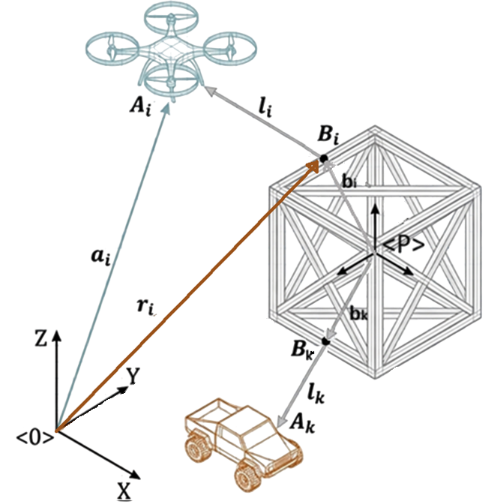
\includegraphics[width=0.5\linewidth]{images/platform_framework.png}
    \caption{Graphical representation of the platform}
    \label{fig:platform_connection_graphical_representation}
\end{figure}

Given the payload twist $^0\xi = \begin{bmatrix}
    ^0v_p & ^0\omega_p
\end{bmatrix}^\top$ in the inertial reference frame $<0>$, we can write the position and velocity of the attachment point $B_i$ (resp. $B_k$) of the aerial vehicle (resp. ground) in $<0>$.
\begin{equation}
    ^0\boldsymbol{r}_i = ^0\boldsymbol{p} + \, ^0_PR \, ^P\boldsymbol{b}_i
\end{equation}
where $b_i$ is the attachment point on payload.
\begin{equation}
    ^0\dot{\boldsymbol{r}}_i = ^0\boldsymbol{v}_p + ^0\boldsymbol{\omega}_p \times \left( ^0_PR \, ^P\boldsymbol{b}_i \right)
    \label{eq:attachmentpointvelWRTinertialframe}
\end{equation}

For definition, the cable vector is $\boldsymbol{l}_i = \boldsymbol{a}_i - \boldsymbol{r}_i = A_i - B_i$ with $\boldsymbol{a}_i$ being the anchor position. 
Under a centralized controller, the positions of all UAV $A_i$ and UGV $A_k$ are known, which directly determin the anchor vector $\boldsymbol{a}_i$. Furthermore, he payload's position and orientation are assumed to be known.ogether with the known locations of the attachment points relative to the payload, this information allows us to calculate the cable vectors $\boldsymbol{l}_i$.

The final form of cable vector variation is given by applying Equation \ref{eq:attachmentpointvelWRTinertialframe} in its definition:

\begin{equation}
    \dot{\boldsymbol{l}}_i = \dot{\boldsymbol{a}}_i - \dot{\boldsymbol{r}}_i = \dot{\boldsymbol{a}}_i - \frac{d}{dt}\left(\boldsymbol{p} + \, _PR \, ^P\boldsymbol{b}_i \right) =\dot{\boldsymbol{a}}_i - \left(\boldsymbol{v}_p + \boldsymbol{\omega}_p \times \left( _PR \, ^P\boldsymbol{b}_i \right)\right)
\end{equation}


Each $\dot{l}_i$ corresponds to the projection of the relative velocity of $B_i$ along the cable direction
\begin{equation}
\begin{aligned}
    \dot{l}_i 
    &= u_i^\top \left( 
        \dot{\boldsymbol{a}}_i 
        - \left( 
            \boldsymbol{v}_p 
            + \boldsymbol{\omega}_p \times (\, _P R \, ^P\boldsymbol{b}_i ) 
        \right) 
    \right) \\
    &= u_i^\top \dot{\boldsymbol{a}}_i 
    - 
    \begin{bmatrix}
        u_i^\top & (\, _P R \, ^P b_i \times u_i )^\top
    \end{bmatrix}
    \xi \\
    &= J_{a,i}\, \dot{a}_i - J_{p,i}\, \xi ,
\end{aligned}
\label{eq:cablelengthrate}
\end{equation}
This gives us the kinematic model that relates the variation of cable length vector $\boldsymbol{\rho}$ with the change in position of the anchors and the payload twist:
\begin{equation}
    \dot{\rho} = J_a \dot{a} - J_p \xi = J_a \begin{bmatrix}
        \dot{a}^{(a)} \\ \dot{a}^{(g)}
    \end{bmatrix} - J_p \xi
    \label{eq:kinematic_model}
\end{equation}

Let $m = n_a + n_g$ be the total number of winches (or cables) and $u_i = l_i/\|l_i\|$ the unit cable direction , then:
\begin{itemize}
    \item $\dot{\rho} = \begin{bmatrix}
        \dot{l}_1 & \dot{l}_2 & \dots & \dot{l}_m
    \end{bmatrix}^\top$ is the cable length rate (dimension $[m\times1]$). 

    \item $J_a$ is the Jacobian relating the anchor velocities to the cable-length rates $[m\times3m]$. In particular, each cable depends only on its anchor velocity.
    
\begin{equation}
J_a =
\begin{bmatrix}
u_1 & 0   & \cdots & 0 \\
0   & u_2 & \cdots & 0 \\
\vdots & \vdots & \ddots & \vdots \\
0 & 0 & \cdots & u_{n_a + n_g} \\
\end{bmatrix},
\qquad
u_j = \frac{(a_j - r_j)}{\|a_j - r_j\|}.
\label{eq:cableVector}
\end{equation}
    \item $J_p$ is the Jacobian relating the payload twist to the cable-length  $[m\times6]$
\end{itemize}
\begin{equation}
    J_p =
\begin{bmatrix}
u_1^\top & \left( \, _pR\, ^pb_1 \times u_1 \right)^\top \\ 
\vdots & \vdots \\
u_m^\top & \left( \, _pR\, ^pb_m \times u_m \right)^\top \\
\end{bmatrix}
\label{eq:jp}
\end{equation}
\begin{note}
    Equation \ref{eq:cablelengthrate} contains $m$ equations in 6 unkown. I need at least six independent cable directions ($\text{rank}(J_p) = 6$).
\end{note}

\noindent The control allocation matrix maps the actuator inputs (cable tension vector) to the system (payload) wrench. For this definition $J_p^\top$ is the allocation matrix.
\begin{equation}
    W_p = J_p^\top \tau
\end{equation}
Let $W_p^*$ being the desired payload wrench, the control allocation problem to solve is
\begin{equation}
    J_p^\top \tau = W_p^*, \qquad \text{s.t}. \tau_i > 0
\end{equation}

\subsection{Static model}
Let $\tau=[\tau_{uav}^\top, \tau_{ugv}^\top]^\top\in \mathbb{R}^{m\times 1}$ the cable tension vector, then
\begin{equation} 
\begin{aligned}
    \underbrace{\tau^\top\dot{\rho}}_{\text{total cable power}} &= \underbrace{\tau^\top J_a\dot{a}}_{\text{UAVs and UGVs mechanical power}} - \underbrace{\tau^\top J_p \, \xi}_{\text{payload power}} \\
    &= (J_a^\top \tau)^\top \dot{a} - (J_p^\top \tau)^\top \xi\\
    &= F_a^\top \, \dot{a} - W_p^\top \, \xi
\end{aligned}
\end{equation}

Each cable $i$ applies a force on the payload $F_{a, i}$ and an equal and opposite force on the UAV (resp. UGV). We can write balance equation on our elements:

\subsubsection{Payload Balance}
\begin{equation}
    \underbrace{W_p}_ {J_p^\top \tau } + \underbrace{W_g}_{\begin{bmatrix}
        0 \\0 \\ - m_p g \\ 0\\ 0\\ 0\\
    \end{bmatrix}} + W_{contact}
 + \underbrace{W_{wind}}_{\parbox{2cm}{\centering let = 0}} = 0
 \label{eq:payloadbalance}
\end{equation}
where since each cable produces a wrench on the payload, the contribution given by the $i$-th cable is:
\begin{equation}
    \underbrace{w_{p,i}}_{6\times 1} = \underbrace{J_{p,i}^\top}_{6\times1} \, \underbrace{\tau_i}_{1\times 1}  = \begin{bmatrix}
        u_i^\top & (\, _P R \, ^P b_i \times u_i )^\top
    \end{bmatrix}^\top \tau_i = \begin{bmatrix}
        \tau_i u_i \\ (\, _P R \, ^P b_i \times \tau_i u_i )
    \end{bmatrix}
\end{equation}
and $W_{contact} = 0$ when there is no contact with the environment.

\subsubsection{UAV balance} % at the attachment point $A_i$
\begin{equation}
    -F_{a,i} + F_{prop, i} + \underbrace{F_{g,i}}_{\begin{bmatrix}
        0 \\ 0 \\ - m_{i} g
    \end{bmatrix}} = 0
    \label{eq:uavbalance}
\end{equation}
with $^iF_{prop} = \begin{bmatrix}
        0 & 0 & F_{prop,z,i}
    \end{bmatrix}^\top$ and $F_{a, i} = J_{a, i}^\top \tau_i = \tau_i u_i$.

UAVs must always generate sufficient thrust to maintain flight and ensure their own stability. As a result, only a portion of their available thrust can be allocated to payload manipulation, which reduces the effective force that can be transmitted through the cables.

\subsubsection{UGV balance}
\begin{equation}
    -F_{a,j} + \underbrace{F_{ground, j}}_{\begin{bmatrix}
        F_{frict,x,j} \\ F_{frict,y,j} \\ F_{norm}
    \end{bmatrix}} + \underbrace{F_{g,j}}_{\begin{bmatrix}
        0 \\ 0 \\ - m_{j} g
    \end{bmatrix}} = 0
    \label{eq:ugvbalance}
\end{equation}
with $\|F_{frict}\| \le \mu F_{norm}$ and $F_{norm} = m_j g - F_{a, z, j}$ and $F_{a,j}$ is obtained through Equation \ref{eq:Fai}.

Similarly, UGVs are subject to ground interaction constraints. In particular, they must satisfy friction limits to remain stationary when no motion is commanded. This imposes bounds on the admissible cable forces, as excessive tension may cause slipping.


\noindent By Newton's third law, the force the cable exerts on the drone $F_{a, i}$ (resp. on the UGV $F_{a, j}$) is equal and opposite to the force it exerts on the payload. Since $u_i$ points from $B_i$ toward $A_i$, the cable pulls the drone with
\begin{equation}
    F_{a, i} = J_{a, i}^\top \tau_i = \tau_i u_i
    \label{eq:Fai}
\end{equation}
As a consequence, the total cable force on the payload is:
    \begin{equation}
        F_p = -\sum_{i=1}^{n_a} F_{a, i} -\sum_{j=n_a + 1}^{n_a + n_g} F_{a, j}
        \label{eq:ForceOnPayload}
        \end{equation}
where the payload wrench is $W_p = \begin{bmatrix}
    F_p & M_P
\end{bmatrix}^\top$

\begin{figure}
    \centering
    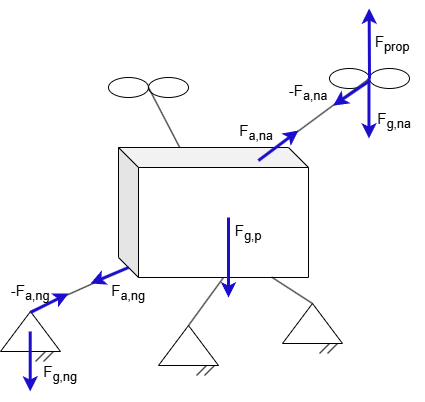
\includegraphics[width=0.5\linewidth]{images/force_on_system.png}
    \caption{Forces acting on the ACTS}
    \label{fig:forceonACTS}
\end{figure}

\subsection{Kinemato-static model}
Writing Equation \ref{eq:payloadbalance}, \ref{eq:uavbalance} and \ref{eq:ugvbalance} in term of $\tau$, we obtain:
\begin{equation}
    W_{sys} = \begin{bmatrix}
        W_p \\ F_a
    \end{bmatrix} = 
    \begin{bmatrix}
        J_p^\top \\ J_a^\top
    \end{bmatrix} \tau = G\tau = \begin{bmatrix}
        -W_g - W_{contact} - W_{wind} \\
        F_{prop} + F_{ground} + F_g
    \end{bmatrix}
\end{equation}
where $F_{prop,j} = 0$ for the UGVs and $F_{ground, i} = 0$ for the UAVs. Then $W_{sys}$ is $(6+3m)\times 1$ and
\begin{equation}
    G\tau + \begin{bmatrix}
        W_g + W_{contact} + W_{wind} \\
        - F_{prop} - F_{ground} - F_g
    \end{bmatrix} = 0
\end{equation}

\section{Mechanical design choices}
\subsection{Payload attachment strategy}
The ACTS consists of at least one UAV, required as the payload needs to be lifted from the ground, and one UGV, included for safety and operational constraints. To fully control the payload in space, we need at least six cables

The configuration of the UAV connections is crucial as it directly affects how forces are applied to the payload.
UAVs are responsible for generating the lifting force required to lift the payload. Consequently, the number of UAVs depends strongly on the payload mass. However, increasing the number of UAVs leads to higher power consumption and greater system complexity. So, adding more UAVs does not necessarily improve performance. 
Additionally, each UAV can be connected to the payload using either a single cable or multiple cables. The choice of configuration affects controllability, wrench feasibility, robustness, and energy efficiency, and should be evaluated accordingly. A practical compromise is to use three UAVs connected to the payload at distinct attachment points, providing a balance between the metrics just mentioned (Figure \ref{fig:uav-possible-configuration}). 

In contrast, UGVs do not contribute to lifting the payload, meaning the same stability arguments do not apply. If we treat the UGVs as fixed anchor points, connecting a single UGV to multiple hook points on the payload simplifies to a standard fixed-anchor scenario. Because each actuator operates independently, this configuration adds no extra mathematical complexity. However, if the UGVs are actively moving, multi-cable connections require precise winch coordination to ensure all cables remain taut at all times. In Figure \ref{fig:UGV_configuration}, possible payload hook attachment can be found.

\todo[inline]{minimum number of cables, redundancy, one cable vs multiple cables}
Since the system is designed to be redundant, the overall number of UAVs and UGVs must be carefully selected.

\subsection{Cable and attachment configurations}
Purpose: Which design variables can actually be changed?

For example: number of UAVs, number of UGVs, number of cables, attachment point locations, cable routing, anchor placement

These are all configuration variables.

Then explain the main alternatives.

UAV configurations
\begin{itemize}
    \item one UAV, multiple cables vs multiple UAVs, one cable each
    \item Pros and cons.
\end{itemize}


Ground attachment configurations
\begin{itemize}
    \item Stewart-like
    \item distributed anchors
    \item asymmetric layouts
\end{itemize}

Payload hook placement
\begin{itemize}
    \item close hooks
    \item spread hooks
    \item influence on torque generation
    \item influence on conditioning
    \item influence on wrench feasibility
\end{itemize}

Cable routing
\begin{itemize}
    \item crossed cables
    \item uncrossed cables
    \item adjacent routing
    \item diagonal routing
\end{itemize}

"These choices define the architecture search space explored in the remainder of the thesis."

\begin{figure}
    \centering
    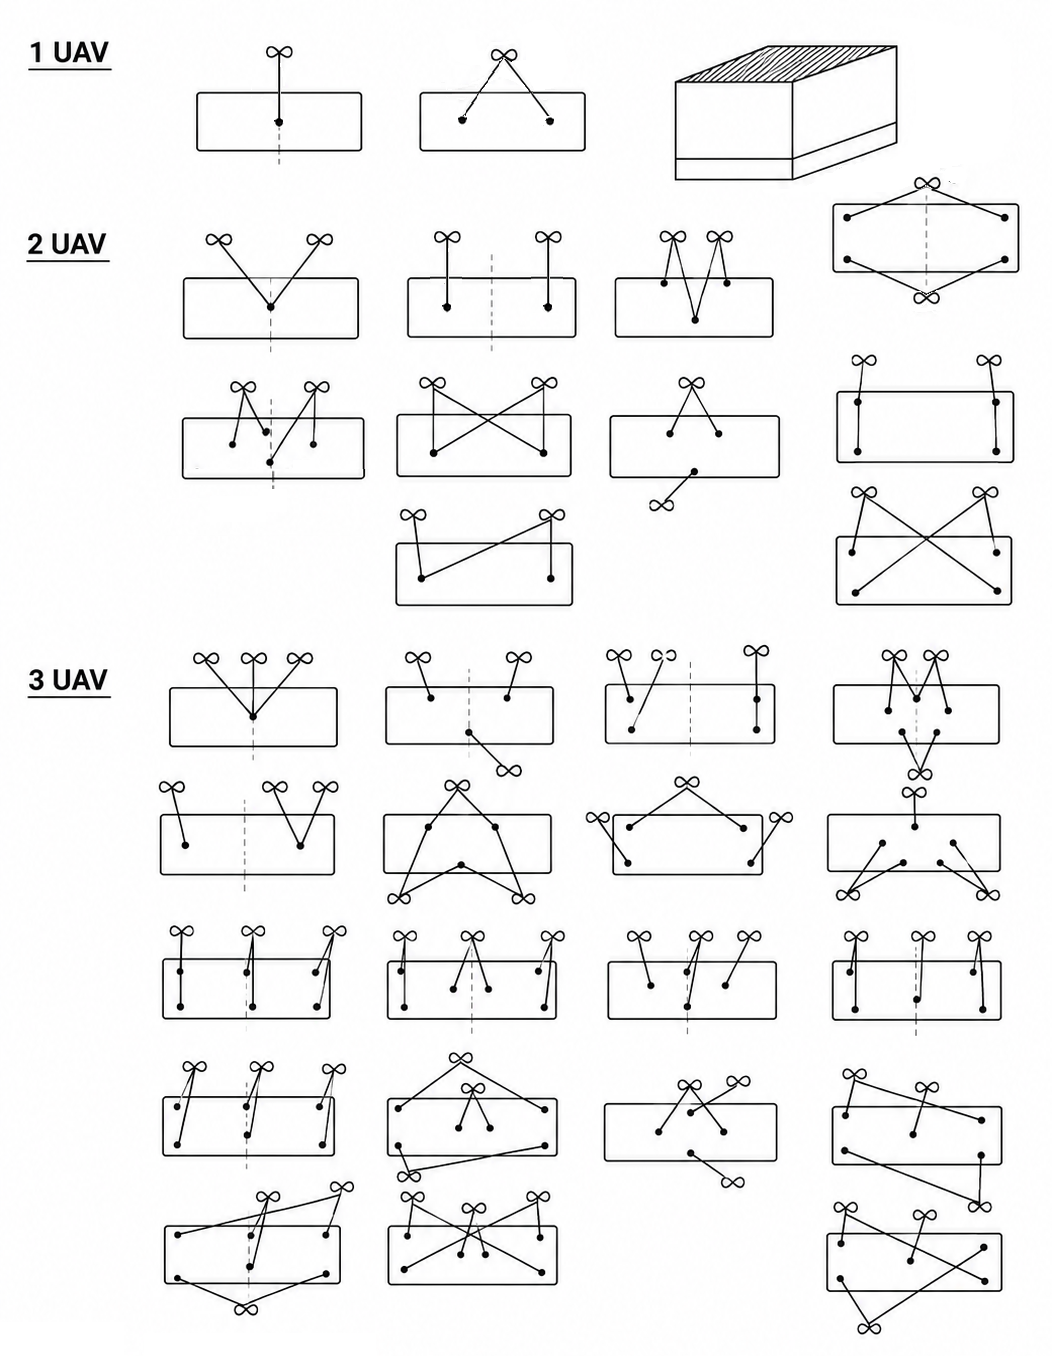
\includegraphics[width=0.58\linewidth]{images/uav_config.png}
    \caption{Possible UAVs connection to the payload}
    \label{fig:uav-possible-configuration}
\end{figure}

\begin{figure}
    \centering
    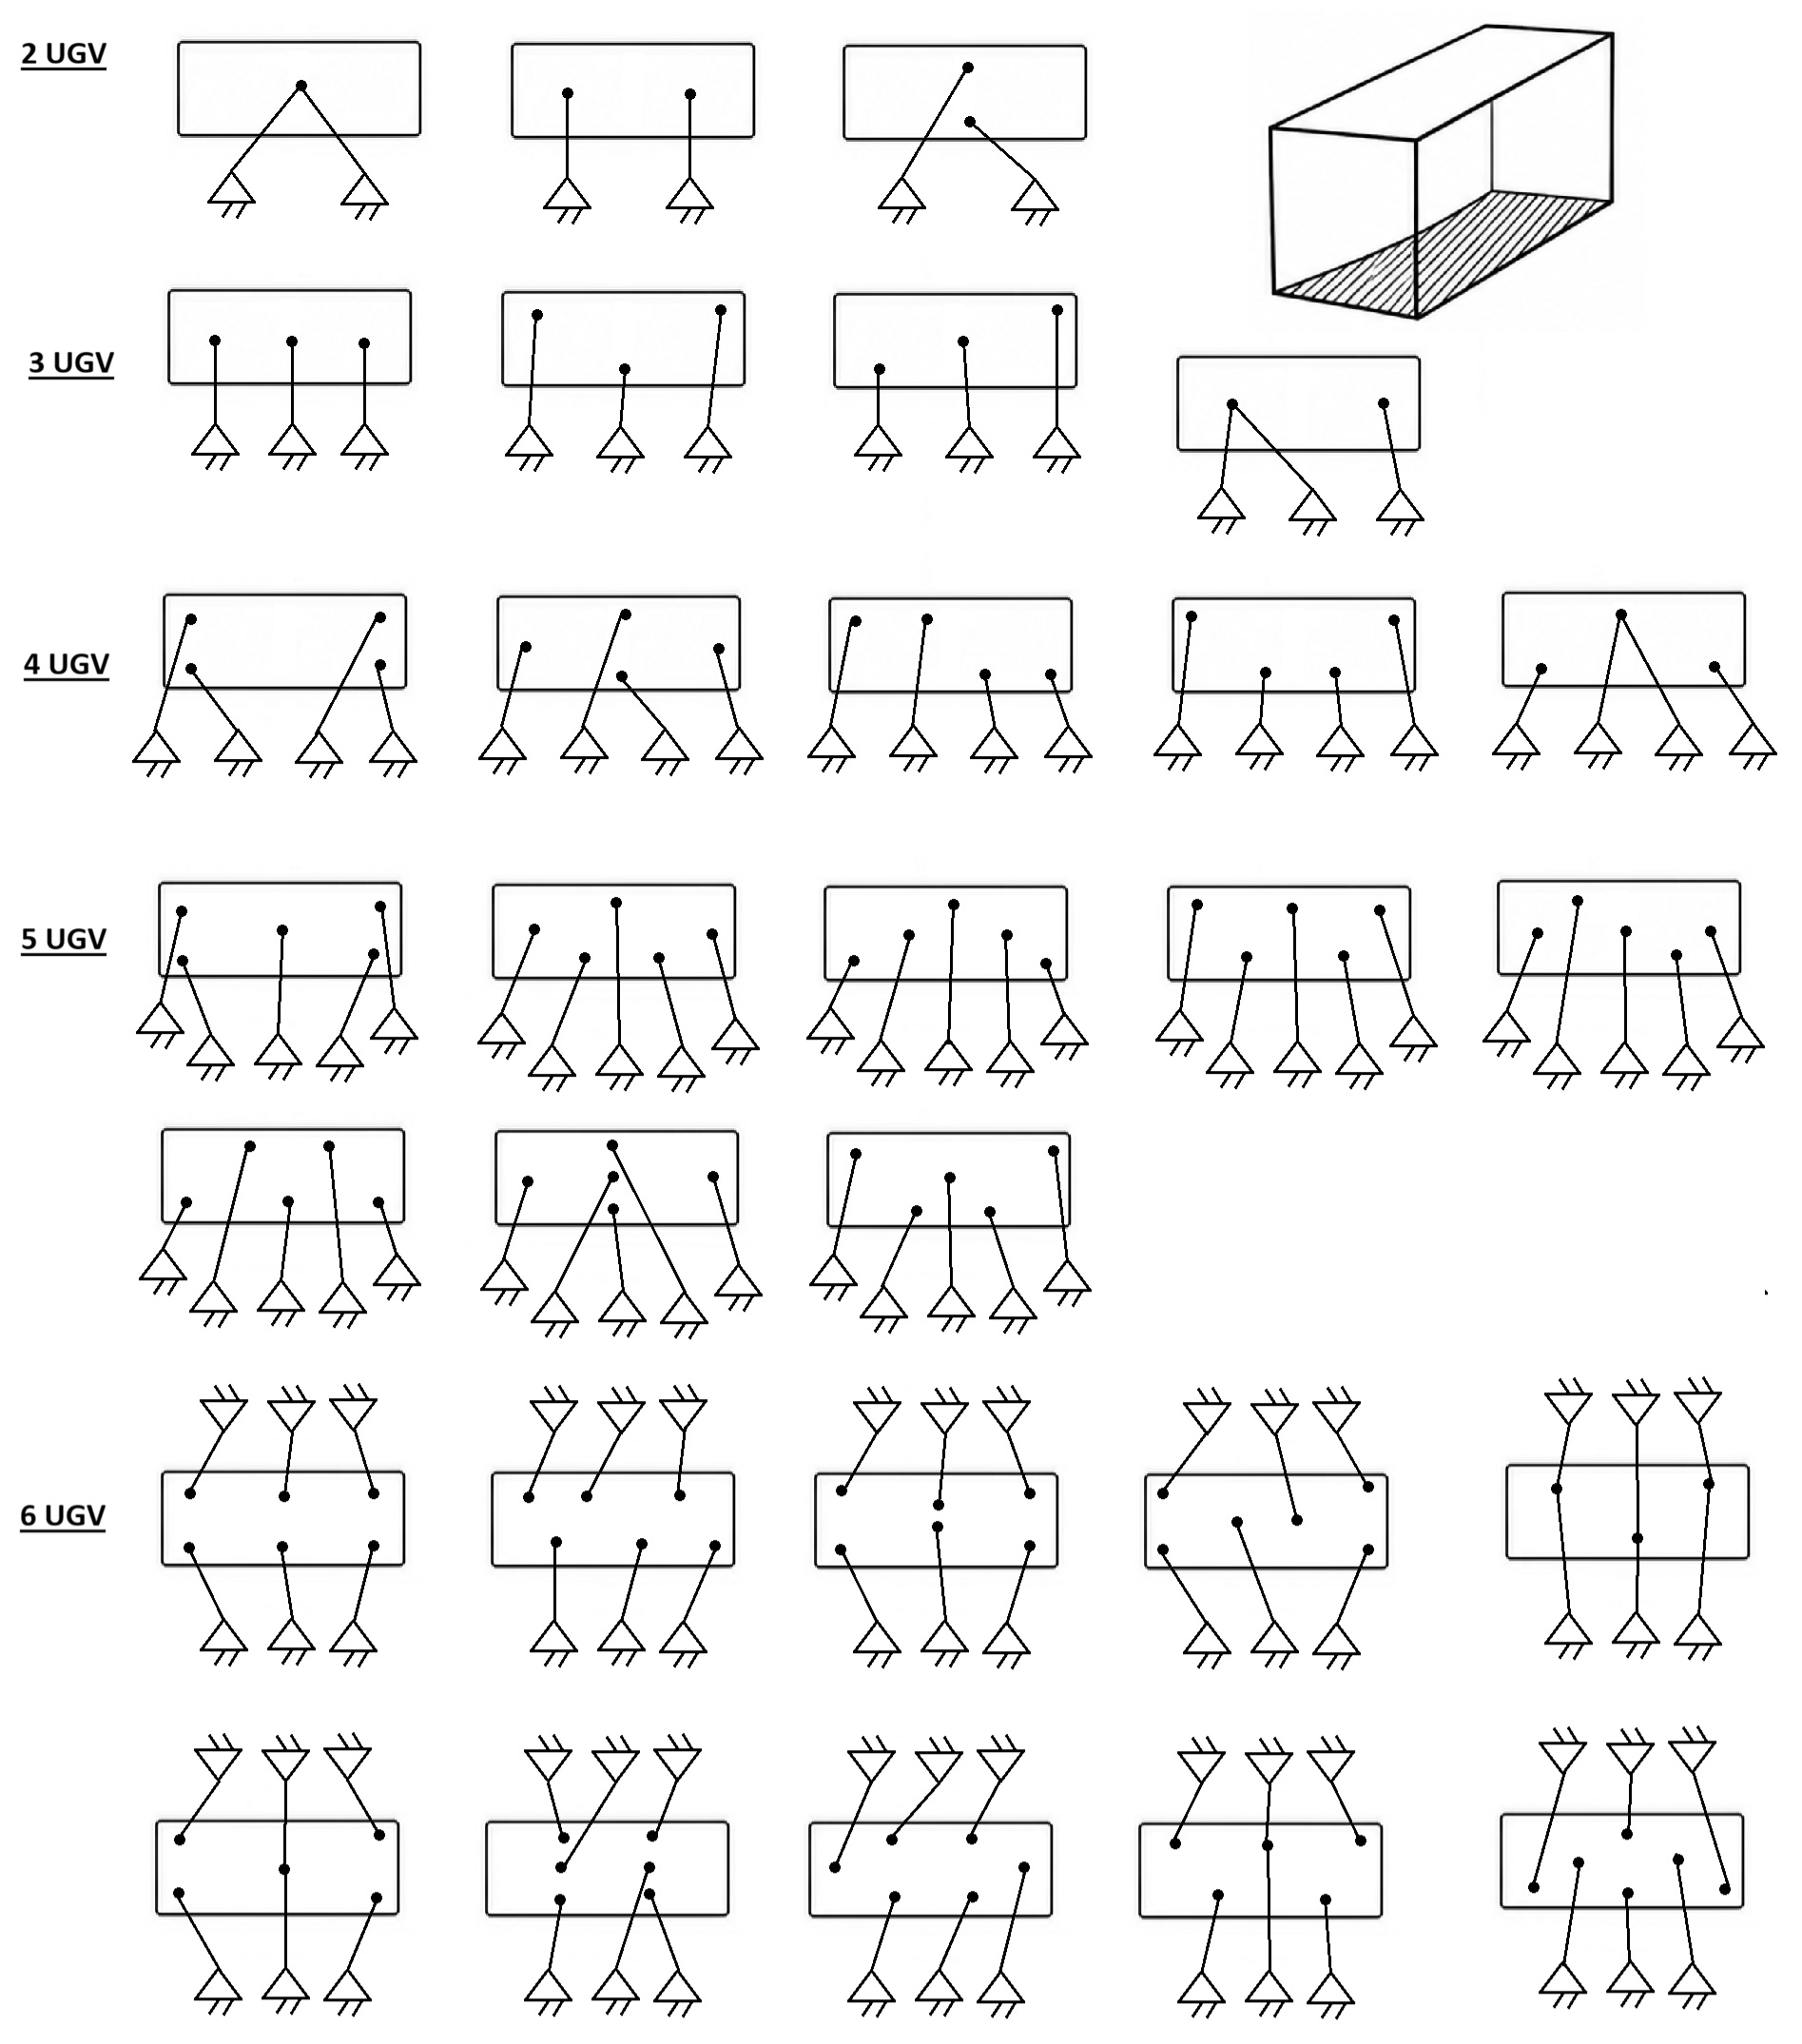
\includegraphics[width=0.58\linewidth]{images/ugv_config.jpeg}
    \caption{Possible UGVs connection to the payload}
    \label{fig:UGV_configuration}
\end{figure}



\newpage


\section{Architecture selection}

\subsection{Performance Indices}
\label{sec:performanceIndices}
In the context of the ShieldBot project, we are working with two questions:
\begin{enumerate}
    \item Which attachment geometry gives the best ability to generate the required payload wrench over the entire mission workspace?
    \item Given the chosen architecture, where should the actuators (UAVs and anchor points in the ground) be positioned and what cable lengths should be used during operation?
\end{enumerate}

\noindent In both cases, we need an objective measurement that guides us in the selection.

\noindent Every configuration to be eligible needs to satisfy feasibility metrics first, such as \cite{cheng_cable_2023}:
\begin{itemize}
    \item Wrench closure conditions (WCC), which guarantees that the payload is fully constrained and arbitrary wrenches can be generated. Mathematically:
    $
    \text{rank}(J_p) = 6
    $
    and positive tensions exist.
    \item Wrench Feasible Condition (WFC), which checks whether tensions remain in the feasible bound $0\le \tau_{\text{min}} \le \tau \le \tau_{\text{max}}$, included UAV thrust limits, cable strength limits and UGV friction limits in a future where the ground anchor point will be movable.
    \item Interference-Free Condition (IFC), ensuring that there is no cable rubbing and no collision with payload edges. Mathematically:
    \begin{equation}
        \begin{aligned}
            d_{ij} \ge d_{\text{safe}}, \quad &\text{where } d_{ij} = \text{dist} \left(\text{cable } i, \text{cable } j\right) &\forall i, j \\
            d_i \ge d_{safe}, \quad &\text{where } d_i = \min_{s\in [0, 1]} \left( \text{dist} \left(r_i + s(a_i - r_i), P \right) \right) &\forall i 
        \end{aligned}
        \label{eq:IFCconstraint}
    \end{equation}
    where $P$ is the payload geometry and $d_{safe}$ is a clearance threshold.
\end{itemize}

\todo[inline]{check this}
However, assuming that all cable attachment points are on the same face of the payload, the only feasible interference between the latter and one of the cables is a near-tangent cable that touches that face. This requirement will be assumed to always be met, as this study places the ACTS in a scenario where this corner case is rarely encountered.

After passing the feasibility filters, we need a way to assign a score to each hook configuration.

\subsubsection{Capacity margin or minimum degree of constraint satisfaction}
The capacity margin is a robustness index that is used to analyze the degree of feasibility of a configuration. It is defined as the shortest signed distance from the task wrench to the boundary of the available wrench set (AWS). Mathematically, it is the minimum of the distances of each one of the $n$ vertex $w_{e, j}$ to each one of the $p$ facet $\left( \mathbf{a}_l, b_l\right)$ of the AWS.
\begin{equation}
    \gamma = \min_{j = 1 \div n} \, \min_{l = 1\div p} \gamma_{j, l}, \quad \text{where } \gamma_{j, l} = \frac{b_l - w_{e, j}^\top \mathbf{a}_l}{\|\mathbf{a}_l\|_2}
\end{equation}
where $\mathbf{a}_l$ is the normal vector to the $l$-th facet and $b_l$ is its offset \cite{pott_arachnis_2015}.

\subsubsection{Worst-Case Capacity Margin}
Additionally, we can define the worst-case capacity margin as how far the system remains from actuator saturation in the most demanding operating condition. Mathematically:
\begin{equation}
    \zeta = \min \left(1 - \max_i \frac{\tau_i}{\tau_{i, max}} \right)
\end{equation}

For each drone, the maximum available cable tension $t_{i, max}$ is based on its maximum thrust $f_{i, max}$ and its current orientation relative to the cable \cite{erskine_wrench_2019}
\begin{equation}
t_{i, max} = m_i \boldsymbol{u}_i^T (\boldsymbol{g} - \ddot{\boldsymbol{x}}_i) + \sqrt{f_{i, max}^2 + m_i^2 \left( \left( \boldsymbol{u}_i^T (\ddot{\boldsymbol{x}}_i - \boldsymbol{g}) \right)^2 - \ddot{\boldsymbol{x}}_i^T \ddot{\boldsymbol{x}}_i - \boldsymbol{g}^T \boldsymbol{g} \right)}
\end{equation}
Considering only quasi-static motion, this can be reduced to the following, where $u_{iz} = \begin{bmatrix} 0 & 0 & 1 \end{bmatrix} \boldsymbol{u}_i$ and $g = \begin{bmatrix} 0 & 0 & 1 \end{bmatrix} \boldsymbol{g}$.
\begin{equation}
    t_{i, max} = m_igu_{iz} + \sqrt{f_{i, max}^2 + m_i^2 g^2 \left(u_{iz}^2 - 1 \right)}
\end{equation}

\subsubsection{Radius of Available Wrench (rAw)}
The radius of the available wrench (rAW) is the maximum magnitude of force that the system can generate uniformly in all directions while remaining within admissible tension limits \cite{jamshidifar_static_2020}. Its optimization helps identify arrangements that simultaneously maximize force robustness, geometric and collision-avoidance constraints, resulting into an enlargement of the static workspace \cite{jamshidifar_static_2020}.

\begin{equation}
    rAW = \min_i \left( \min \left(\frac{|d_{pi}|}{\|\mathbf{n}_{null, i} \|}, \frac{|d_{qi}|}{\|\mathbf{n}_{null, i} \|} \right)\right)
\end{equation}
being $u_{null, i} = \text{null}(M_i)$ with $M_i$ containing combinations of linearly independent cable unit vectors and $d_{pi}$ and $d_{qi}$ defined as:
\begin{equation}
    \begin{aligned}
        d_{pi} &= \sum_{j \in I^+} \tau_{max} u_{nulli}^T u_j + \sum_{j \in I^-} \tau_{min} u_{nulli}^T u_j - m |u_{nulli}^T g| \\
        d_{qi} &= -\sum_{j \in I^-} \tau_{max} u_{nulli}^T u_j - \sum_{j \in I^+} \tau_{min} u_{nulli}^T u_j - m |u_{nulli}^T g|
    \end{aligned}
\end{equation}
However, since \cite{jamshidifar_static_2020} consider the case of a point-mass payload, it does not take in consideration the torques, we may compute separately rAW$_{force}$ and rAW$_{moment}$, the maximum pure force (resp. torque) the platform can exert in any direction while generating zero net moment (resp. linear force).


\subsubsection{Conditioning index}
The conditioning index measures how uniformly the system can generate forces and moments in different directions. Mathematically:
\begin{equation}
    \nu = \frac{\sigma_{\min}(J_p)}{\sigma_{\max}(J_p)} \in [0, 1]
\end{equation}
$\sigma_{\min}$ and $\sigma_{\max}$ are the minimum and maximum singular values of the Jacobian matrix, obtained via Singular Value Decomposition (SVD) \cite{erskine_dynamic_2021}. A small conditioning number indicates a well-conditioned system, far-away from singular configuration.

\subsubsection{Manipulability}
The manipulability index, defined as $w = \sqrt{\text{det}(J_pJ_p^\top)}$, measures the volume of the wrench ellipsoid. A value close to 0 means that the system hit a kinematic singularity, while large value means a large overall wrench generation capability.

\subsection{Selection Strategy}
\todo[inline]{update it with what we are actually using}
\todo[inline]{Say that this is an option but then just announced which one we used, but it will be talken better in the next chapter}
Once the feasibility constraints are satisfied, we may want to proceed either by
\begin{equation}
    N =w_1 \hat{\gamma} + w_2 \,  \hat{\text{rAw}} + w_3 \hat{\zeta}
\end{equation}
where all the metrics are scaled to $[0, 1]$, or either choosing the solution that maximizes the radius of available wrench between all the solutions that satisfy $\gamma > \gamma_{\text{min}}$ and using the worst-case capacity margin as a tie breaker.

Our solution will finally be:
\begin{equation}
    U^* =\arg \max_U \left(N(U) \right)
\end{equation}

\subsection{Selected architecture}
We are interested in working with an over-actuated system. Therefore, we will start using six cables for fully control the payload pose and three drones acting as an anti-gravitational force. A schematic is shown in Figure \ref{fig:6cables3dronesSchem}. 


\begin{figure}[h]
    \centering
    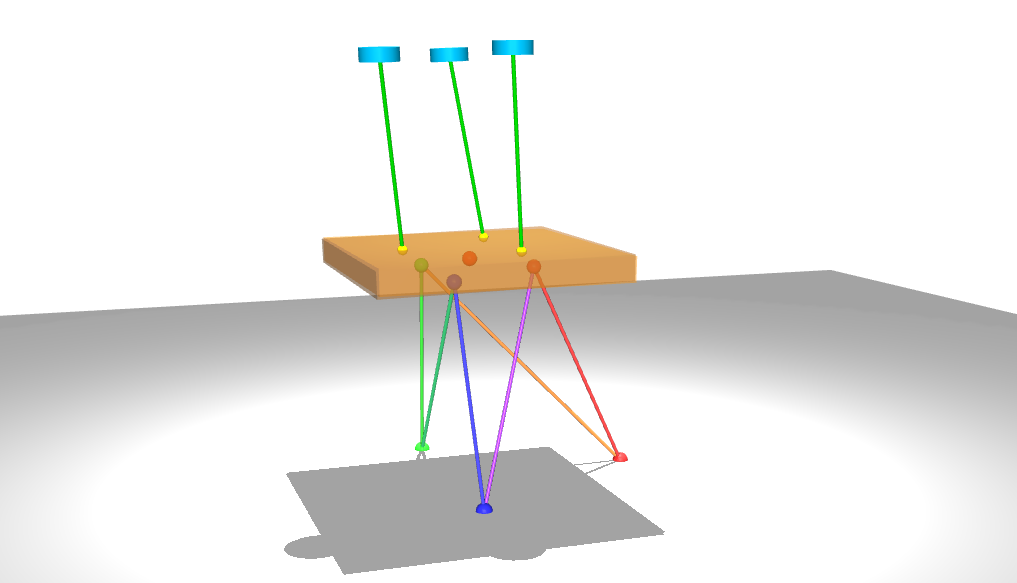
\includegraphics[width=0.8\linewidth]{images/acts_stewart_mujoco.png}
    \caption{Over actuated ACTS with 6 ground cables and 3 UAVs}
    \label{fig:6cables3dronesSchem}
\end{figure}
